\appendix
\chapter{Additional Experiments}
Some more text ...

% \section{\gpp usage}
% \label{appendix:corpus-phonemizer-usage}

% \lstset{basicstyle=\small\ttfamily}
% \begin{lstlisting}[float=tp, breaklines=true,caption={An extract taken from the help menu of \gpp, displaying the tool's usage.}]

% usage: corpus_phonemizer.py [-h] [-k] [-v] [-u] [-i INPUT_FILE]
%        [-o OUTPUT_FILE] {epitran,phonemizer,pingyam,pinyin_to_ipa} language

% Phonemize utterances using a specified backend and language.

% positional arguments:
%   {epitran,phonemizer,pingyam,pinyin_to_ipa}
%                                         The backend to use for phonemization.
%   language                              The language to phonemize.

% options:
%   -h, --help                            show this help message and exit
%   -k, --keep-word-boundaries            Keep word boundaries in the output.
%   -v, --verbose                         Print debug information.
%   -u, --uncorrected                     Use the wrapper's output without
%                                         applying a folding dictionary to correct
%                                         the phoneme sets.
%   -i INPUT_FILE, --input-file INPUT_FILE
%                                         Input file containing utterances (one
%                                         per line). If not specified, reads from
%                                         stdin.
%   -o OUTPUT_FILE, --output-file OUTPUT_FILE
%                                         Output file for phonemized utterances.
%                                         If not specified, writes to stdout.

% Example usage:
%   python corpus_phonemizer.py epitran --language eng-Latn --keep-word-boundaries --verbose < input.txt > output.txt
% \end{lstlisting}

% \section{Corpus Phonemizer Folding Dictionaries}
% \label{appendix:folding-dictionaries}

\section{Average Information Density of Transcribed Child-Directed Speech Increases with Age Cross-Lingually}\label{app:parentese}

The phonemic representation of the utterances in our dataset open up new avenues for exploring the phonotactic properties of languages and the information-theoretic properties of child-directed speech. %Previous research in these areas have had to base their calculations on word types \citep{piantadosi2011word, dautriche2017words, pimentel2020phonotactic} or orthographic text \citep{mahowald2013info, dautriche2017wordform, futrell2020lossy}, often citing a lack of phonemic data as a limiting factor. %For instance, \citet{piantadosi2011word} show a strong correlation between information and word length across 10 languages using orthographic data, stating that orthographic word length is correlated with phonetic length, but this may not be the case for certain languages. 

%This representation may be useful when comparing languages that have different levels of orthographic transparency (the correspondence between how words are written and how words are pronounced). 

\begin{figure}
    \centering
    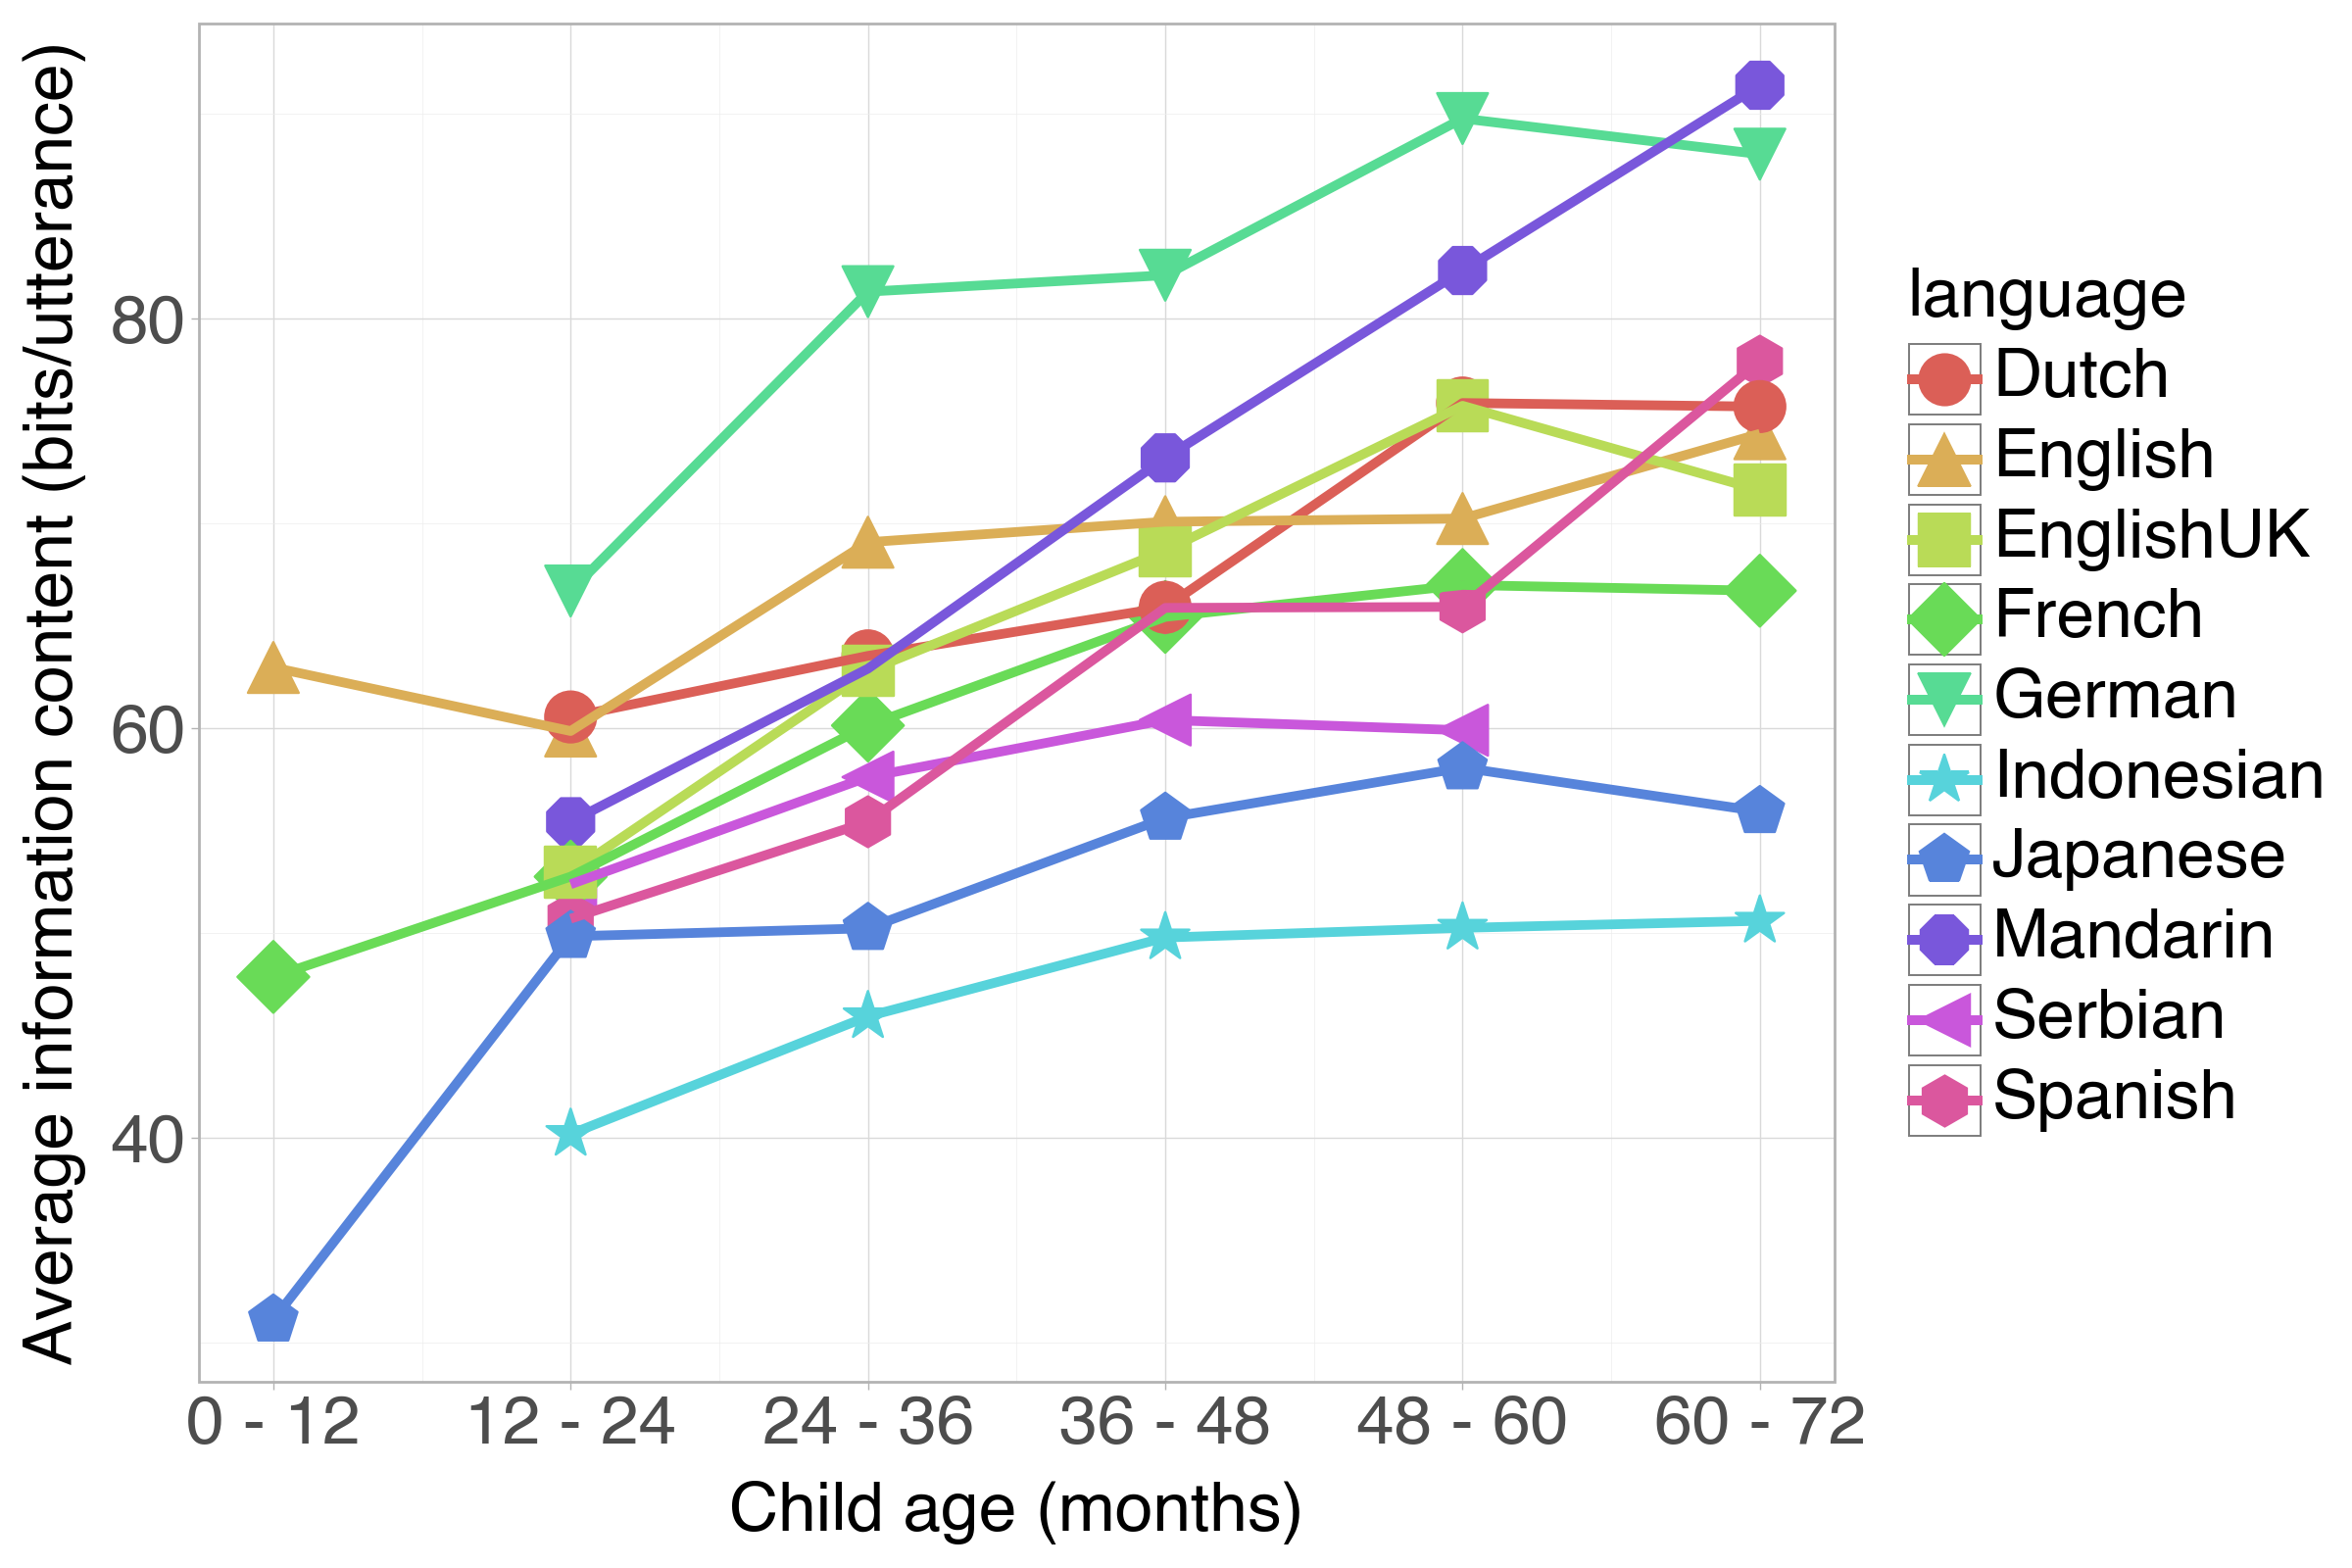
\includegraphics[width=0.99\linewidth]{13Resources/information-trends.png}
    \caption{Average information of child-directed utterances in CHILDES}
    \label{fig:13-information-trends}
\end{figure}

Here, we demonstrate one information-theoretic experiment, comparing the average information content of child-directed utterances to the age of the child being spoken to (this information is also available in CHILDES and is preserved in our dataset). We group child ages in years (0-12 months, 12-24 months, etc.) and calculate the average information content of a sample of child-directed utterances using a unigram language model. The information $I_U$ of each utterance consisting of a sequence of phonemes $p_1,p_2,\ldots,p_n$ is given by

$$I_U = -\sum_{i=0}^{n}{log_2P(p_i)},$$

where $P(p_i)$ is the probability of phoneme $p_i$ given by its frequency in the data. We plot the average information of utterances in each age category for the largest 10 languages in the dataset in \cref{fig:13-information-trends}. We find that across all 10 languages the average information of utterances increases with the age of the child, indicating that speakers of `Parentese' may adjust the complexity of their speech according to the learner's age. 

\chapter{Implementation Details}\label{app:implementation}

We conduct our experiments using the \texttt{PyTorch} framework \citep{paszke-etal-2019-pytorch} and the \texttt{Transformers} library \citep{wolf-etal-2020-transformers}.

\subsection{Hardware Details}

We use a server with one NVIDIA A100 80GB PCIe GPU, 32 CPUs, and 32 GB of RAM for all experiments. Below, we report a subset of the output of the \emph{lscpu} command:

\begin{tcolorbox}[left=5pt,right=5pt,top=5pt,bottom=5pt]
\small
\begin{verbatim}
Architecture:        x86_64
CPU op-mode(s):      32-bit, 64-bit
Address sizes:       46 bits physical, 
                     48 bits virtual
Byte Order:          Little Endian
CPU(s):              32
On-line CPU(s) list: 0-31
Vendor ID:           GenuineIntel
Model name:          Intel(R) Xeon(R)
                     Silver 4210R CPU
                     @ 2.40GHz
CPU family:          6
Model:               85
Thread(s) per core:  1
Core(s) per socket:  1
Socket(s):           8
Stepping:            7
BogoMIPS:            4800.11
\end{verbatim}
\end{tcolorbox}


\subsection{Model Parameters and Training Procedure}

\begin{table}[ht!]
    \centering
    \small
    \begin{tabular}{lc}
    \toprule
         Parameter & Value\\
    \midrule
         Layers & 12 \\
         Heads & 12 \\
         Dropout & 0.1 \\
         Embedding Size & 768 \\
         Inner Size & 3072 \\
         Max Example Length & 128 \\
         Learning Rate & 0.001 \\
         Optimizer & AdamW \\
         Scheduler Type & Linear\\
         Max Steps & 400,000 \\
         Warm-up Steps & 90,000\\
         Per Device Batch Size & 32 \\
    \bottomrule
    \end{tabular}
    \caption{Hyperparameter settings for training the GPT-2 architecture. Vocabulary size varies according to the tokenizer used, but all other parameters are constant across experiments. Where values are not reported, they may be assumed to be default values.}
    \label{table:baseline_hyperparams}
\end{table}

We describe the model and training parameters in \cref{table:baseline_hyperparams}. The model parameters were chosen to match those of the Pythia-170M model from the Pythia suite \citep{biderman2023pythia}. The model has 85M non-embedding parameters and is also equivalent in size to GPT-Neo 125M and OPT-125M. The Pythia models use the GPTNeoX architecture which is slightly different to GPT-2. In initial experiments, we found that GPT-2 performed better on the benchmarks across all eight of our conditions. 

Data is prepared into batches by first tokenizing the entire dataset, combining all tokens into one long vector, and then splitting the vector into chunks of 128 tokens. Only the very last example is padded, if required. At each step during training, random chunks are selected and combined into batches. 

Checkpoints are taken every 50,000 steps during training. At each checkpoint, the perplexity is evaluated on the held-back evaluation set, and at the end of training the checkpoint with the lowest perplexity is returned as the best model. 